% \section{Background on NLP}
\subsection{Tasks}\label{sec:tasks}
NLP research is mostly driven by the basic question, how do humans understand the natural language and how can we make the machines do the same? In the research, understanding the natural language for machines differs from lower level problems of extracting information from the text like named entity or relation extraction to higher level problems like machine translation or question answering. In this section we will discuss about the different kind of tasks involved in NLP dividing them into three broad categories:

\begin{enumerate}
    \item Extraction
    \item Generation
    \item Summarisation
\end{enumerate}

\subsubsection{Extraction}
Knowledge Extraction is a sub field of NLP that deals with the automated extraction of structured knowledge from unstructured sources. These are the few examples of the tasks that can be treated as knowledge extraction.

\paragraph{Named Entity Recognition}
Named Entity Recognition is the a sub task of Knowledge Extraction that deals with identifying the various entities in a piece of text such as person, location, organization and date. It has various use cases, like automating hiring process or optimizing the search engine algorithms. One of the main approach is to use BIO notation (B for beginning, I for inside and O for non-entity tokens.) For example, in the sentence \textit{`Boris Johnson won the UK general elections'} the entities can be marked as $[Boris]_{B-PER}$ $[Johnson]_{I-PER}$ $[won]_{O}$ $[the]_{O}$ $[UK]_{LOC}$ $[general]_{O}$ $[elections]_{O}$. PER represents person, LOC represents location and O is the non-entity tokens.

There are various open source libraries for NER such as spaCy which uses hand crafted features (not published) and StanfordNLP which uses a combination of hand crafted features and deep learning for the same task. One of the most popular benchmark for NER is CoNLL 2003 \cite{sang2003introduction} consisting text from news wires like Reuters dataset tagged in four different categories (PER, LOC, ORG, MISC). The state-of-the-arts in literature for NER right now are mostly based on the transformers architecture which we will discuss is \cref{sec:transformers}

% NER SRL Chunking sequence tagging
% Named Entity Recognition deals with 

\paragraph{Parts-of-Speech Tagging}
deals with the marking of parts of speech of a word in the text corpus. The category of words having similar grammatical properties can be termed as parts-of-speech. Some of the common parts-of-speech in English language are noun, pronoun, adjective, preposition, verb, adverb etc. NLTK is one of the most common open-sourced library used for POS tagging. A example of POS tagging in NLTK for the sentence \textit{`And now for something completely different'} can be \textit{[('And', 'CC'), ('now', 'RB'), ('for', 'IN'), ('something', 'NN'),
('completely', 'RB'), ('different', 'JJ')]}. Here CC is coordinating conjunction, RB is used for adverbs, IN is a preposition, NN is noun and JJ is adjective \footnote{Example taken from \url{https://www.nltk.org/}}.

The popular benchmarks for POS tagging are Penn Treebank \cite{marcus1993building} and Universal Dependencies \cite{silveira14gold}. Penn Treebank portion of Wall Street Journal (WSJ) consists of 45 different POS tags whereas Universal Dependencies consists of more than 100 treebanks from 60 different languages. The current state-of-the-arts for POS tagging are mostly based on LSTM and BERT.

\paragraph{Natural Language Inference}
For a given piece of text or premise, finding that whether some `hypothesis' about that text is true or not is called natural language inference. If a hypothesis is true then it is known as `entailment', if it is false then `contradiction' and for undetermined `neutral'. For example, lets have a look at the \cref{tab:nli} \footnote{Example taken from \url{https://nlpprogress.com/}}.

\begin{table}[h!]
  \begin{center}
    \caption{NLI Example}
    \label{tab:nli}
    \begin{tabular}{l|c|r} % <-- Alignments: 1st column left, 2nd middle and 3rd right, with vertical lines in between
      \textbf{Premise} & \textbf{Label} & \textbf{Hypothesis}\\
      \hline
      A man inspects the uniform of a & contradiction & The man is sleeping.\\
      figure in some East Asian country. &  & 
    \end{tabular}
  \end{center}
\end{table}

The two most common corpus for NLI are Multi-Genre Natural Language Inference (Multi-NLI) \cite{williams2017broad} and Stanford Natural Language Inference (SNLI) \cite{bowman2015large}. Both of them contain around 500k labelled hypothesis/premise pairs. Current state of the arts are based on the slight modification of BERT architecture.

\paragraph{Relation Extraction}
The task of identifying semantic relationships between entities of text is known as relation extraction. Usually the relations are defined between two or more entities like person, location or organisation and fall under various pre-defined semantic categories.

There are lots of public datasets available for relation extraction and all of them define their own category of relations that need to be extracted from the text. Few examples are; Capturing discriminative attributes (SemEval 2018 Task 10) \cite{krebs2018semeval} where users are asked to identify if a given attribute can help in discrimination between two concepts. Few-Shot Relation Classifier (FewRel) \cite{han2018fewrel} consisting of 70k sentences with 100 different kinds of relation annotated by crowd-sourcing on wikipedia corpus. New York Times corpus \cite{riedel2010modeling} containing entities extracted from NYT corpus and linked to the freebase knowledge base. 
% There are different types of state-of-the-arts based on hand crafted features as well machine/deep learning algorithms to achieve good results on these datasets.

% \paragraph{Template Filling} The approach of efficient extraction and representation of 

% \paragraph{Semantic Role Labelling}


% \paragraph{Dependency Parsing}

\subsubsection{Generation}
Natural Language Generation (NLG) can be termed as the sub-field of NLP which deals with the generation of natural language given some structured or unstructured information. Machine Translation and Data Augmentation can be few examples of NLG.

\paragraph{Machine Translation}
Machine Translation has been one of the most popular problems in NLP. It deals with the translation of text from one natural language to another, for example, translating English text to Hindi or vice-versa. A snippet from Google translate performing MT is shown in fig. \ref{fig:mt_example} \footnote{\url{https://translate.google.com/}}.

\begin{figure}
    \centering
    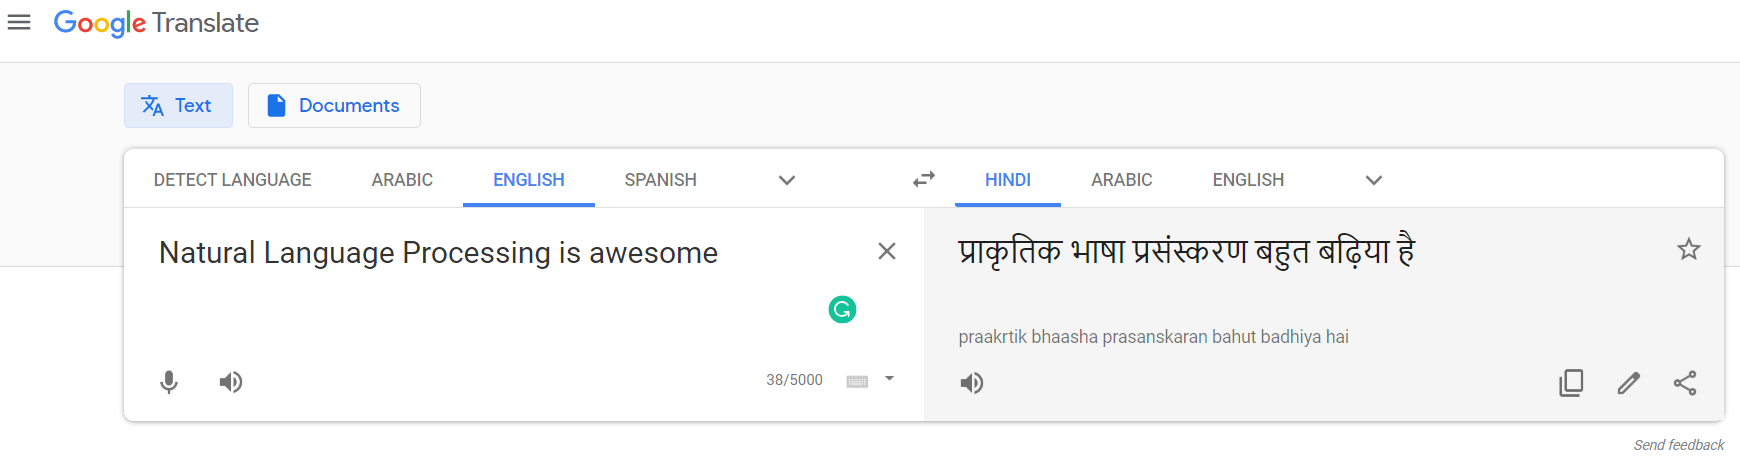
\includegraphics[width=\textwidth]{images/mt.png}
    \caption{An Example of Machine Translation}
    \label{fig:mt_example}
\end{figure}

The MT models are evaluated on the method called BLEU score which is used as the higher the better. Some of the common public datasets availabel are WMT 2014 EN-DE and WMT 2014 EN-FR \cite{bojar-EtAl:2014:W14-33} which contains many english-german and english-french pair of sentences. The current state-of-the-arts are based on mainly transformers and some attention based LSTMs.

\paragraph{Data Augmentation}
With the popularity of Deep Learning based NLP, there has been a huge requirement of training data for building the models. Collecting the labelled data is sometime very costly and take a lot of resource in terms of time and money. 

The alternative way of getting more data is to generate a huge corpus of data by tweaking the using the small amount of training data available in some fashion. This technique is known as data augmentation. The way of tweaking differs from problem to problem. There are different ways of data augmentation like unsupervised back translation with consistency training \cite{Xie2019} or contextualized word replacement \cite{kobayashi2018contextual}.

\subsubsection{Summarisation}
The third category of NLP tasks is termed as the problem of summarisation. Given a piece of text, how can we summarize the information it posses in simpler and/or structured manner. 

\paragraph{Text Classification}
Classifying a piece of text/document into some pre-defined categories can be termed as the task of text classification. Text classification is mainly used in applications like sentiment analysis and/or topic and document classification. 

For example, in sentiment analysis we try to identify the sentiment or polarity of a sentence based on its content. Given a review about a product on Amazon and identifying if the customer who wrote the review is positive or negative about the product's quality. Some of the common examples for topic classification can be identifying the domain (political, religious or technological) of a news article based on its content.

Some popular datasets for sentiment analysis are; imdb movie reviews which contains 50,000 reviews of different movies from imdb website labelled into positive and negative classes. They also contain a numeric value from 1 to 10, 1 being the lowest rating and 10 being the highest rating. The current state-of-the-art is XLNet based on the transformer architecture for this \cite{yang2019xlnet} dataset.

Another famous dataset for text classification is Dbpedia dataset which consist of 5.6M labelled texts from the 14 non-overlapping topics of wikipedia. BERT \cite{devlin2018bert} is the current best performing algorithm with only 0.64 error rate on this dataset.

\paragraph{Question Answering}
Question Answering is a token-level task of NLP where given a piece of information with some question related to it, the system needs to generate an acceptable answer for it. One of the most famous dataset for this task is Stanford's Question Answering Dataset (or SQuAD) which consists of different questions asked by users of wikipedia related to some wikipedia article. The answer to this question is a segment from the same article only. The current state-of-the-arts for this datasets are the ensemble models based on different versions of BERT. An updated leaderboard for this dataset can be found on their website \footnote{\url{https://rajpurkar.github.io/SQuAD-explorer/}}.

% \paragraph{Aspect-Based Sentiment Analysis}

% \paragraph{Summary Generation}
% Chat-bots in NLP are very popular in today's world. They can interact with the users in a very humane manner and are very efficient. Suppose, a company has to interact with their customers on the website on the daily basis. One way to answer the queries of these customers will be have support assistants hired to answer these queries as the part of their job. But this can be very expensive. On the other hand, the company can use an automated software to do the same job if 